\documentclass[11pt]{article}
\usepackage[utf8]{inputenc}
\usepackage{amsmath}
\usepackage{amsfonts}
\usepackage{amssymb}
\usepackage{graphicx}
\usepackage[super]{nth}
\usepackage{amsthm}
\usepackage{bm}
\newtheorem{theorem}{Theorem}
\newtheorem{objective}{Objective}
\newtheorem{model}{Model}
\usepackage{xcolor}
\definecolor{light-gray}{gray}{0.95}
\newcommand{\code}[1]{\colorbox{light-gray}{\texttt{#1}}}
\usepackage{listings}
\usepackage{placeins}

\usepackage[authoryear]{natbib}


\makeatletter
\renewcommand{\maketitle}{
\begin{center}

\pagestyle{empty}

{\LARGE \bf \@title\par}
\vspace{1cm}

{\Large Marcel Gietzmann-Sanders, Michael Courtney, Andrew Seitz, Curry Cunningham}\\[1cm]

University of Alaska Fairbanks


\end{center}
}\makeatother


\title{Probabilistic Deep Learning as a Framework for Progressive Development of Behavior Models}

\date{2024}
\setcounter{tocdepth}{2}
\begin{document}
\maketitle



\section*{Introduction}

We begin with a specific motivating example - animal movement. Animal movement can be modeled as a discrete Markov process by discretizing the environment into a grid. At each time step, the animal's movement can be represented as a decision, $d_i$, among a set of possible choices, $c_{i,j}$, where each choice corresponds to a grid cell the animal might reasonably move to given its current location. Then, with information about these choices, $\vec{v}_{i}$, the model would predict the conditional probability $P(c_{i,j} | \vec{v}_{i})$ - the likelihood of the animal moving to a specific grid cell in the next time step.

This approach differs from the more common practice of predicting specific movement parameters \citep{mlmovement1}, such as step lengths and turning angles, by instead focusing on probabilities across discrete options. This provides a key advantage in that even early-stage models with limited predictive power can still provide valuable insights. Models predicting specific movements require high precision to avoid compounding errors during simulation, probability-based models, on the other hand, allow for broader applications by tracking how an individual's probability mass spreads across potential trajectories over time. This flexibility enables model developers to deliver meaningful results early on, using available data, while continuing to refine and improve predictions as more information becomes available.

This process of progressive development is further strengthened by leveraging early models as tools for exploratory data analysis (EDA). Because the model assigns a likelihood to each choice and trajectory, it can highlight specific decisions, individuals, locations, or time periods where the predicted likelihoods are unusually low compared to the rest of the data. These act as exemplars for further study. Additionally, as new models are developed, comparing likelihoods across versions can reveal what each model captures — or fails to capture — about the system. This makes the modeling process not only predictive but also a dynamic tool for uncovering patterns, refining hypotheses, and identifying areas that warrant deeper investigation.

The kind of progressive development described here is only feasible if the process of building and refining models - beyond the initial feature engineering - is quick and efficient. Iterative modeling and EDA become impractical if each iteration demands significant time and effort. Such efficiency can be enabled by recognizing that the framing proposed here is largely equivalent to that of a probabilistic deep learning classification task \citep{durr} - which enables developers to leverage the automation inherent in deep learning. Taking advantage of machine learning also means the tools used at one stage in the development are the same throughout the model's development - all that changes are the features input. 

Each of the advantages described above — early value in development, utility in exploratory data analysis (EDA), and automation through machine learning — are not new to movement modeling. Hidden Markov Models, for example, inherently provide conditional probability distributions \citep{mlmovement1}, much like the framing presented here, and several movement models have been developed using machine learning \citep{mlmovement1}\citep{mlmovement2}\citep{mlmovement3}. However, the Markov models usually rely on explicit assumptions about the interaction between data and behavior, limiting their flexibility and integration with machine learning. Conversely, many machine learning models focus on explicit predictions of movement rather than offering likelihoods across all options. The value of the framework proposed here lies in its ability to combine these advantages, enabling progressive development through early value, application in EDA, and automation through machine learning. 

Finally, while this application of probabilistic deep learning has so far been couched in the context of modeling movement, the framework — selecting among discrete choices — has the potential for broad applicability across a range of organism behaviors. The only requirement is the ability to represent the behavior in question within this discrete, choice-based structure.

Given the potential of probabilistic deep learning as a framework for progressively developing animal behavior models, this paper has two primary objectives, and is organized as follows. (1) to provide a guide in overcoming some of the practical challenges that arise in applying probabilistic deep learning to behavioral data and (2) to provide an illustrative example, using Chinook salmon movement data, of how exploratory data analysis derived from the modeling process itself can be used to drive further model developments. With this guide, motivating example, and the accompanying code available at https://github.com/networkearth/mimic, it is hoped that this framework will help catalyze an iterative mode of discovery.

\section*{Guidance on Applying the Technique}

\subsection*{Theory}

Standard probabilistic deep learning networks are typically framed as a classification problem, using categorical cross-entropy as the loss function \citep{durr}. Using such a loss function amounts to minimizing the negative log likelihood across the examples in the training data. Each output neuron represents a potential choice, with the model predicting the probability of each choice being correct based on this loss formulation. For these choices, we provide the network with features encapsulating the relevant information. Training is then comprised of providing a series such decisions. 

However, this formulation introduces a critical challenge: if there are $N$ features per choice and $M$ potential choices, the overall dimensionality of the input space becomes $N \cdot M$. Adding even a single feature increases the dimensionality by $M$ not just 1.

This growth poses a significant challenge due to the "curse of dimensionality", where the amount of data required to effectively train models can grow exponentially with the dimensionality of the input space \citep{curse}.

\subsection*{Log-Odds Modeling}

To address this issue we could take advantage of the order invariance of choices in the traditional framing. In other words the order in which choices are presented to the model should not matter. For instance, whether a particular choice appears in the first or the thirteenth position should have no impact on the model's operation. This property allows for data augmentation by reordering choices. In essence, for each training example, $M!$ (factorial of the number of choices) augmented examples can be created.

The issue with this approach is that as your augmented data size grows to match the needs of the greater dimensionality, so too does the time required for training. So while the problem remains theoretically possible, the potential exponential uptick in time complexity poses a significant practical issue. \newline

\begin{figure}[h!] 
	\centering
  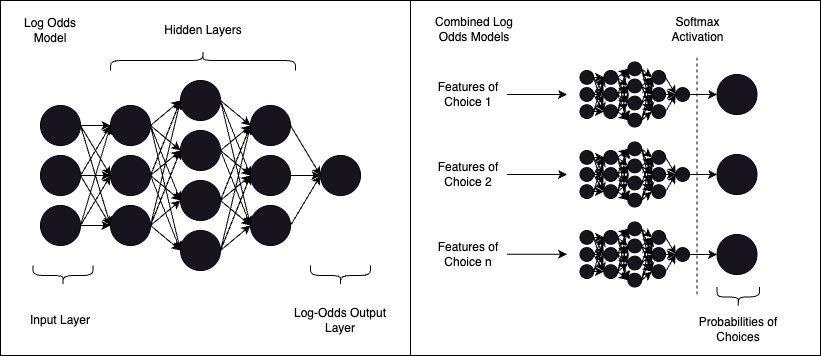
\includegraphics[height=55mm]{figures/log_odds.png}
  \caption{Log-Odds Model: Each choice is passed through a log odds model (left) whose output is then passed through a softmax layer whose weights are fixed in order to produce probabilities that can be passed to a categorical cross entropy loss function. By sharing weights between choices we effectively reduce the dimensionality of the problem. }
  \label{fig:log_odds}
\end{figure}

\FloatBarrier


Instead we propose an adjustment to the standard framing of probabilistic machine learning. Instead of predicting the probabilities directly, we predict the log-odds $\phi_m$ for each choice and calculate the probability $p_m$ using the softmax function:

$$p_m = \frac{e^{\phi_m}}{\sum_{m=1}^{M}e^{\phi_m}}$$

This approach reduces the feature space dimensionality to $N$ and effectively increases the number of training examples by a factor of $M$.

We can implement this log-odds model using standard probabilistic deep learning techniques by replicating the "log-odds model" weights across all $M$ choices (Figure \ref{fig:log_odds}). The outputs are fed into a softmax layer with $M$ units, where the layer's weights are set to the identity matrix and biases are set to zero. Using categorical cross-entropy as the loss function ensures compatibility with standard probabilistic deep learning while enabling us to train the log-odds weights and significantly reduce the problem's dimensionality.

\subsection*{Contrast Sampling}

A practical issue with our log-odds framing is that as $M$ grows large most instances of the internal log-odds model would ideally report very low log-odds, resulting in low probabilities. Ideally, only one choice should produce $p_m=1$. This is analogous to a class imbalance problem, where the model becomes prone to predicting the most common class.

To address this, we balance the training data. Instead of presenting the model with full decisions containing all $M$ choices, we create training pairs, or contrasts, where each pair consists of one selected choice and one unselected choice. This approach is valid because the log-odds model focuses on the relative likelihood of choices, making the number of choices considered at any one time irrelevant.

The primary risk in using contrasts is introducing bias by disproportionately sampling certain combinations of choices. To mitigate this, we randomly sample pairs from each decision, ensure an equal number of contrasts per decision, and an equal number of decisions per individual. This preserves the balance across the training data and avoids skewing the model's learning.

\subsection*{Taking Advantage of the Cloud}

Finally, in deep learning the specific layer sizes, depth, optimizer, learning rate, and other parameters best suited to a particular problem are not usually known from the start. Therefore it is important to do hyperparameter tuning in order to discover the best parameters for a particular problem. Practically this means training large numbers of models - a process that is usually very compute intensive. Even with just 3 parameters 5 distinct values each results in 125 distinct models. Furthermore as with any search over a non-convex space, the initial seed can have impacts on the final solution. Therefore, training deep learning models requires training many models per problem.

This challenge can be overcome by virtue of the fact that these models can all be trained independently and therefore in parallel. This is a perfect use case for cloud compute where one can spin up, for a short time and a reasonable cost, a large number of machines and do all of the hyperparameter tuning in parallel. A primary benefit of the code at https://github.com/networkearth/mimic is to help do exactly this. 

\subsection*{Summary}

In summary the steps in applying log-odds modeling are:

\begin{enumerate}
\item Discretize the behaviors into distinct decisions $d_i$ and choices $c_i,j$. 
\item Resample the choices using contrast sampling
\item Apply log-odds modeling to the contrasts, taking advantage of cloud compute to efficiently search the hyperparameter space
\item Use the trained model to make inferences on the original decisions (as opposed to the contrasts)
\end{enumerate}

\section*{Application to Chinook Salmon Movement Data}

\subsection*{Outline}

With this guide in hand we will proceed to demonstrate this technique by building three, very simply, models of Chinook salmon (\textit{Oncorhynchus tshawytscha}) movement. These specific models build on one another and were chosen to illustrate how one might use this technique as an exploratory data analysis (EDA) tool. The features for each model are as follows (the + indicating the model takes on the features of the model above it in addition to those listed in its row): 

\begin{center}
\begin{tabular}{| c | c  | } 
\hline 
Model & Features \\
\hline
Distance Model & distance to choice \\
Heading Model & + heading to choice \\
Food Model & + primary productivity, mixed layer thickness \\
\hline
\end{tabular}
\end{center}

and their purposes (in terms of EDA) are described here:

\begin{center}
\begin{tabular}{| c | c  | } 
\hline 
Model & Purpose \\
\hline
Distance Model & A null model for comparison \\
Heading Model & Look at heading tendencies in the data \\
Food Model & Explore deviations from averages due to productivity \\
\hline
\end{tabular}
\end{center} 

We will begin by describing the data and associated features, then move onto the specifics of training the models (following our guide), and finally, in the results and discussion, illustrate how the models can be used to explore the data. 

\subsection*{Data and Features}

The data used is a series of tracks from 111 Chinook salmon (\textit{Oncorhynchus tshawytscha}) caught and monitored between 2013 and 2022 \citep{tags1} \citep{tags2}. These tracks were obtained from pop-up satellite archival tags which collect temperature, light level, and depth information at specified (sub day) intervals. This data is then passed through a proprietary algorithm from Wildlife Computers to determine likely longitude and latitude during each day of of monitoring \citep{PSAT}. \newline

\begin{figure}[h!] 
	\centering
  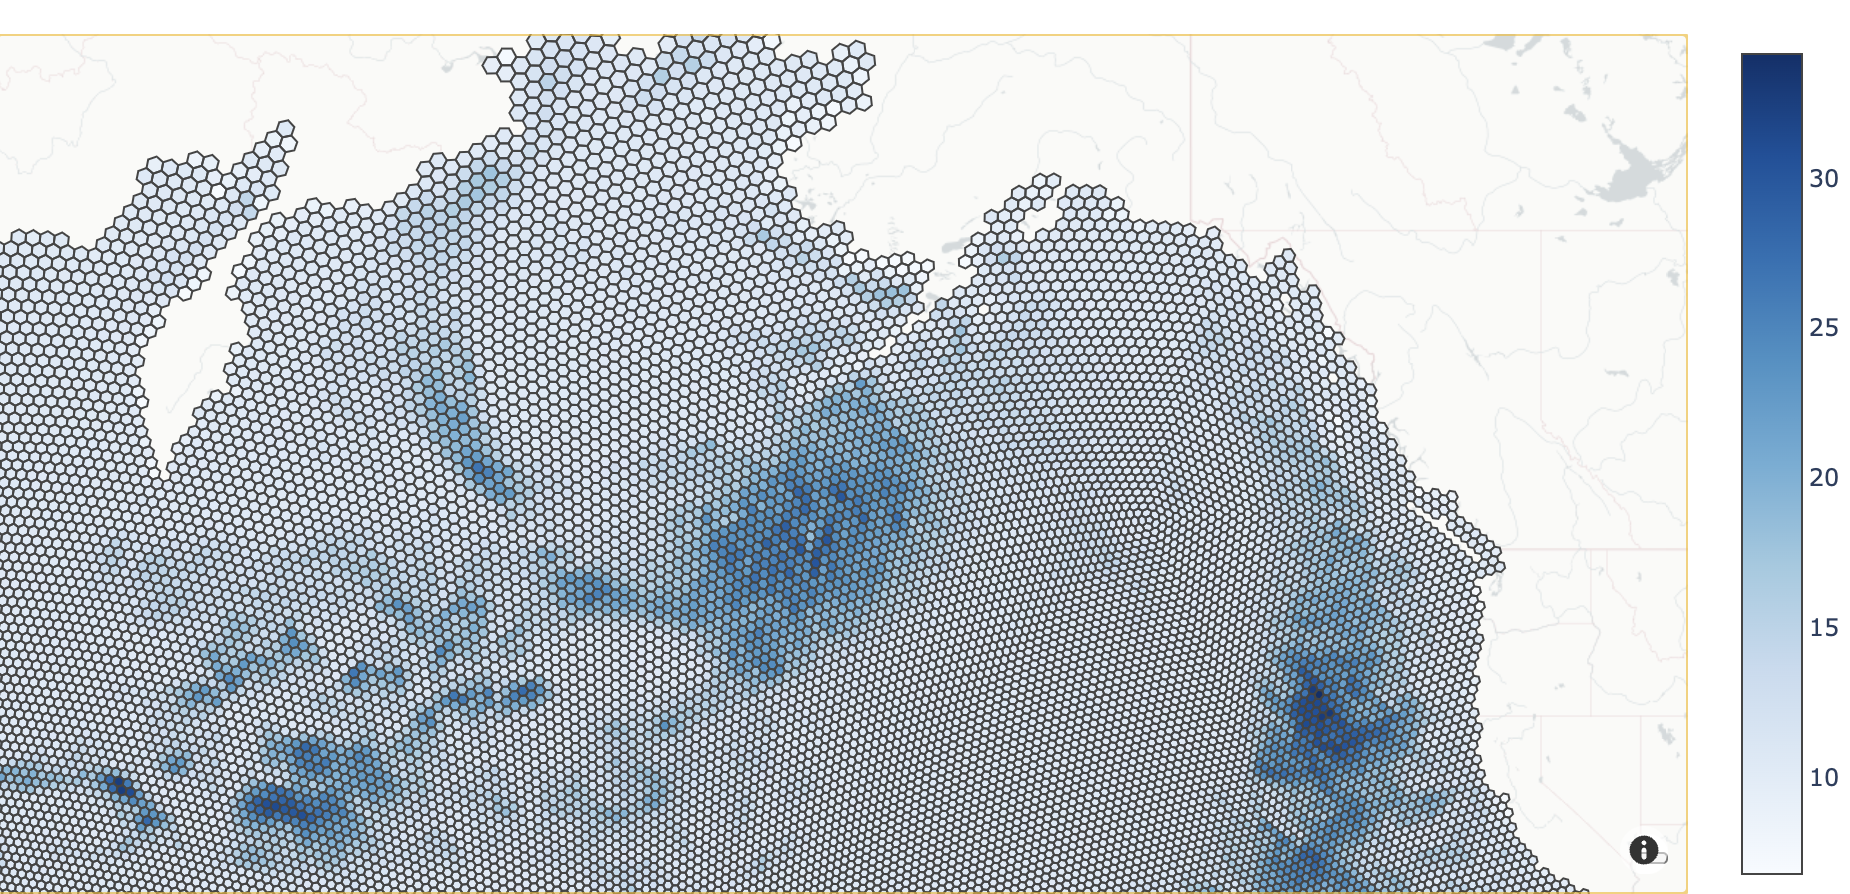
\includegraphics[height=55mm]{figures/mlt_2021_07_02.png}
  \caption{Mixed layer thickness (m) per h3 cell (resolution 4) on July 2, 2021.}
  \label{fig:mlt}
\end{figure}

Environmental data was derived from the Global Ocean Biogeochemistry Hindcast dataset (10.48670/moi-00019) and the Global Ocean Physics Reanalysis (10.48670/moi-00021) from the E.U. Copernicus Marine Service Information. Net primary production (mg/m3/day) and mixed layer thickness (m) were aggregated per Uber h3 resolution 4 cell in the Northern Pacific. As a reference for the resolution of the data see Figure \ref{fig:mlt}. \newline

Movement heading in radians and distance to the centroid of the choice cell were computed. Mixed layer thickness and net primary production were joined to the choices on h3 cell index and day.

Distance was normalized to a range of 0-1 through division by 100, while mixed layer thickness and net primary production were both log-scaled and then centered at zero. 

\subsection*{Building the Models}

\subsubsection*{Train and Validation Sets} 

The first step was to split into training and validation sets. Given the low number of individuals in the sample and the intention to demonstrate the technique's value as an EDA tool it was decided to not maintain a hold out test set.

71 individuals were randomly selected for training and 40 for validation.

\subsubsection*{Formulation}

The next step in building a log-odds model is to decide on the formulation of our choices. In our case we decided to grid space by Uber h3 cells at resolution 4. Specifically, the cell containing each salmon location from our data was identified and then, assuming a maximum travel distance of 100km (centroid to centeroid) all adjacent cells within the 100km were identified as choices (including the currently occupied cell). In general this represented $\sim 19$ choices per decision. As such our model ends up predicting the probability, given the data, of moving to any one of those cells. Training data was derived by identifying the actual cell moved to. 

\subsubsection*{Contrast Sampling}

Next we needed to determine the specifics of the contrast sampling. For this example, after inspecting the distribution of number of choices per salmon and number of choices per decision, we decided on random sampling (with replacement) 200 decisions per individual and 19 choices per decision. 

Over a validation/training split of 40, 71 this resulted in 421,800 contrasts of which 269,800 were used in training and the rest in validation. 

Note that only 14,200 training examples would've been available to a traditional probabilistic approach representing a large increase in the number of available training examples. 


\subsection*{Training and Model Selection}

For each of the three models trained, the hyperparameters for the internal log-odds component of the model were parametrized in the following way:

\begin{center}
\begin{tabular}{| c | c |} 
\hline 
Component & Options \\
\hline
Layers & 3, 4 \\ 
Units per Layer & 24, 32 \\
Batch Size & 10000 \\
Learning Rate & 0.0005 \\
\hline
\end{tabular}
\end{center}

We proceeded by grid search and used 5 separate seeds for each combination. Models were trained in Keras using an Adam optimizer for 100 epochs. Training was done on AWS Batch using Fargate instances of 2 vcpu's and 4 GB of memory. By taking advantage of AWS Batch,  models could be all trained in parallel allowing for short (~1 hour) turn around times. 

Lowest loss (categorical cross entropy) at the end of the 100 epochs over the validation dataset was used to select the best set of parameters for each of the three models trained.


\section*{Results}

The loss, categorical cross entropy, is equivalent to the average (normalized) log probability per contrast. For an equivalent metric over the actual decisions made by the individuals we computed the average log probability per decision for each individual and then computed an average over those across individuals (in order to not favor individuals with many decisions). This is the D-NLP reported in the table below. 

\begin{center}
\begin{tabular}{| c | c | c | c | c |}
\hline 
Model & Train C-NLP & Val C-NLP & Train D-NLP & Val D-NLP \\
\hline
No Model & -0.693 & -0.693 & -2.944 & -2.944 \\
Distance & -0.172 & -0.154 & -1.336 & -1.223 \\
Heading & -0.156 & -0.150 & -1.281 & -1.200 \\
Food & -0.147 & -0.146 & -1.248 & -1.180 \\
\hline
\end{tabular}
\end{center}

"No Model" assumes all decisions are equally likely, "Distance" is the distance only model, "Heading" adds the movement heading, and "Food" adds the net productivity and mixed layer thickness features. \newline

\begin{figure}[h!] 
	\centering
  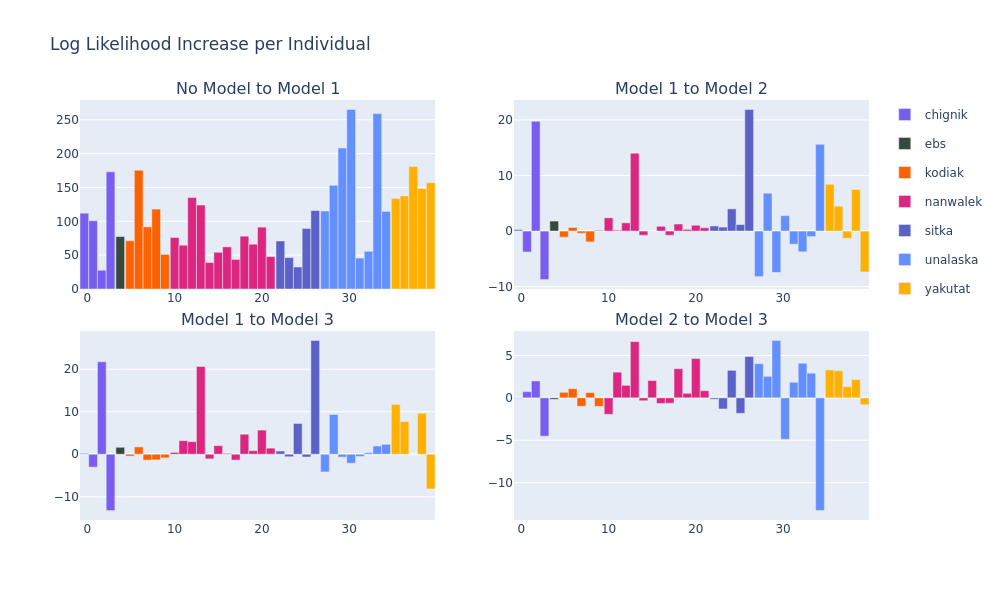
\includegraphics[height=70mm]{figures/ll_increase.png}
  \caption{Log likelihood increase (unnormalized) per individual of each model change.}
  \label{fig:ll_increase}
\end{figure}

\begin{figure}[h!] 
	\centering
  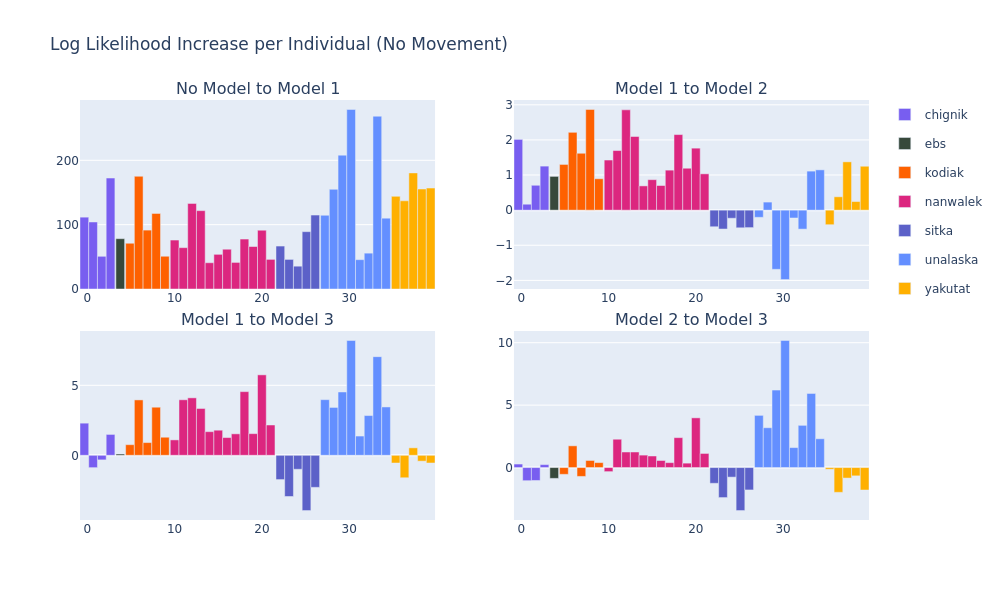
\includegraphics[height=70mm]{figures/ll_increase_no_movement.png}
  \caption{Log likelihood increase (unnormalized) per individual of each model change in cases where the selection involved no movement.}
  \label{fig:ll_increase_no_movement}
\end{figure}

\FloatBarrier

\begin{figure}[h!] 
	\centering
  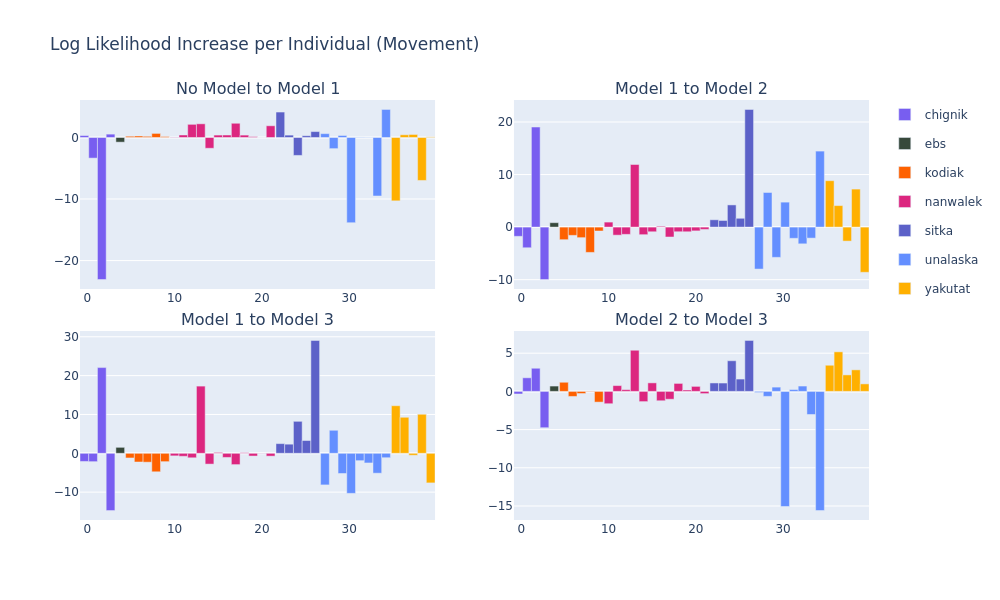
\includegraphics[height=70mm]{figures/ll_increase_movement.png}
  \caption{Log likelihood increase (unnormalized) per individual of each model change in cases where the selection involved movement.}
  \label{fig:ll_increase_movement}
\end{figure}



Figure \ref{fig:ll_increase} shows the unnormalized changes in log likelihood for each individual colored by the region in which they were initially tagged as we go from one model to the next. Figures \ref{fig:ll_increase_no_movement} and \ref{fig:ll_increase_movement} break this down for decisions that resulted in no movement and movement respectively. Only individuals in the validation set were considered.

The appendix contains a series of mapped examples (figures \ref{fig:chignik_map}-\ref{fig:yakutat_map}) from each of these regions (besides EBS) that shows how the log likelihood per decision (when moving) changed in moving from model 1 to model 2 and then from model 2 to model 3. As in the above, only individuals in the validation set were considered.\newline

Finally as much of the behavior seems to be modulated by movement distances (or lack of movement) a summary table of empirical likelihood of movement of a specific distance is given (taken over all individuals). 

\begin{center}
\begin{tabular}{| c | c | c |}
\hline
Distance Bin (km) & Likelihood of Selection & \# Training Decisions \\
\hline
No Movement & 65.6\% & 3163 \\
Up to 50km & 32.5\% & 1567 \\
50km to 100km & 1.9\% & 92 \\
\hline

\end{tabular}
\end{center}


\section*{Discussion}

\subsection*{The Distance Model}


In any probabilistic classification problem model performance has to be evaluated against some kind of "null" baseline. For example in our case, given there are normally 19 choices available in each decision any model must be able to produce likelihoods of selecting the correct choice greater than $1/19\approx 0.05$ on average. Anything below this and a purely random guess is better. 

In our example however a random guesser can be smarter than this without having any information on the environment or organisms in question because there are simple descriptive features that can be derived from the formulation alone. I.e., someone with just those statistics could become an "informed random guesser". In this analysis we look at two of them - distance and movement heading. 

The first, distance, provides a significant drop in our loss from -2.944 in the no model case to -1.223 in the distance model. We can also plot the change in the log likelihood per individual track (figure X) and see that adding distance to the model represents an improvement across every single individual considered. Our random guesser is very usefully informed by the distance associated with each choice and so our "null model" should include this feature. 

\subsection*{The Heading Model}

Next we turn to the model that includes the movement heading per decision as well. Here we also see a shift in the loss but of far lesser magnitude than in going from the no model case to the distance model. Specifically we go from a validation loss of -1.223 to -1.200. While this is useful, far more informative is a comparison plot that shows us the shift in log likelihood per individual track when going from the distance model to the movement heading model (figure X). Unlike the latter figure this one restricts itself to choices where movement occurred. This is our first example of the usefulness of these models in doing EDA as this plot is effectively showing us, per individual, the alignment with average tendencies of movement in the data. 


The individuals with marked positive increases represent individuals well aligned to the movement heading tendencies in the data whereas those quite negatively aligned show a contrary pattern. Using this we can then plot the movements themselves for these "exemplar" individuals colored by their changes in likelihood compared to the distance model (blue is positive, red is negative) to see what those general tendencies in the data are (figure X). From this it is clear that the model is learning a south westerly pattern as being the best direction to randomly guess. 

This is all incredibly useful to the model builder as we are now in possession of exemplars who need little explanation beyond these basic descriptive features as well as specific exemplars that act contrary to the "norm". These individuals can now be studied more extensively to look for discriminating patterns we can use to further improve the model.  

\subsection*{The Food Model}

The examples in yakutat presented an especially interesting example in that the exhibit "low likelihood" behavior at the beginning of their tracks and then switch to higher likelihood behaviors (according to the heading model) later on as they then proceed to move down the coast. This gave the authors a very specific shift to watch and observe for patterns and one pattern seemed to be that when the mixed layer thickness began to shrink the fish began to move south. To see more clearly how these features might interact with the ones already given mixed layer thickness and primary productivity were added and comparisons as before were done (figure X). 

First, the addition of these features did make consistent improvements across individuals' movement choices in the yakutat and sitka groups and much of this improvement was on the tracks south. However these same groups all saw a decline in the likelihood of decisions that resulted in no movement - something that would certainly be worth additional investigation. For unalaska the opposite pattern is seen - decisions that resulted in no movement saw a strong positive increase whereas there were very strong drops in likelihood for movement decisions. The other groups had far more mixed responses. Looking at the specific likelihood changes per movement decision (figure X) in unalaska we see that the likelihoods of decisions in an easterly direction actually dropped as compared to the movement heading model whereas for yakutat the directions that were already boosted by the movement heading model were further boosted by the addition of these features. Clearly understanding these marked differences between the unlaska and sitka and yakutat groups is key to understanding some important aspect of these individuals' movement behavior.

\subsection*{Summary of EDA}

The purpose of these three example models was to show how by using this modeling process and looking at the likelihood changes per individual, decision, or group of choices, the modeling can be used to identify classes of behaviors that warrant additional investigation as well as general tendencies in the data. These kinds of outcomes are precisely the purpose of exploratory data analysis and are essential to building, and understanding, robust models. 

\subsection*{Beyond EDA}

While the primary focus of this example has been directed at the use of probabilistic models as tools for exploratory data analysis, their predictive capabilities should not be overlooked. One of the key strengths of probabilistic modeling lies in its ability to perform well even when the available features are only weakly predictive. By outputting probabilities rather than deterministic predictions, the model can effectively capture uncertainty and express it in a way that is both interpretable and actionable.

In scenarios where features have low predictive power, deterministic models of behavior over time can struggle because of an accumulation of errors. Probabilistic models, on the other hand, distribute probability mass across choices, reflecting the underlying uncertainty in the data. This enables better decision-making under uncertainty, as the model not only identifies the most likely choices but also quantifies the likelihood of alternatives, given the data available.

Moreover, the iterative refinement of these models makes them particularly valuable in predictive contexts. As new information comes to light or existing information is improved there is no need to rebuild or rethink models from scratch, instead the same framework can be used to build the old as well as new models. This allows for faster evaluation, more flexibility and freedom in considering new information, and therefore a better chance of picking features in a purely data driven manner. 

\subsection*{Wide Applicability}

Finally while this example focused on one species - Chinook salmon - and one aspect of behavior - movement - this methodology applies to any problem that can be framed in terms of discreet decisions $d_i$ and choices $c_i,j$. This could include movements of other species such as birds or mammals and other behaviors such as food selection, mating choices, or timing of spawning. By adapting the feature set and decision structure to the system of interest, researchers can reuse the same tools to study a wide variety of different behaviors. 


\subsection*{Conclusion}

This study highlights the dual power of probabilistic machine learning in providing both predictive insights and a robust framework for exploratory data analysis. The log-odds modeling technique exemplifies how dimensionality challenges can be overcome, and along with parallelism in the cloud enables rapid iteration and refinement of models to uncover patterns that would otherwise remain hidden. Ultimately, this framework is more than a predictive tool; it is an investigative lens, empowering researchers to probe the intricacies of behavior and the factors driving it. 


\newpage

\section*{Code}

The tooling used to build these models as well as the means to deploy them using Amazon Web Services has been packaged at: \newline https://github.com/networkearth/mimic

\bibliographystyle{apalike}
\bibliography{reference}
\newpage
\section*{Appendix: Mapped Examples}

\begin{figure}[h!] 
	\centering
  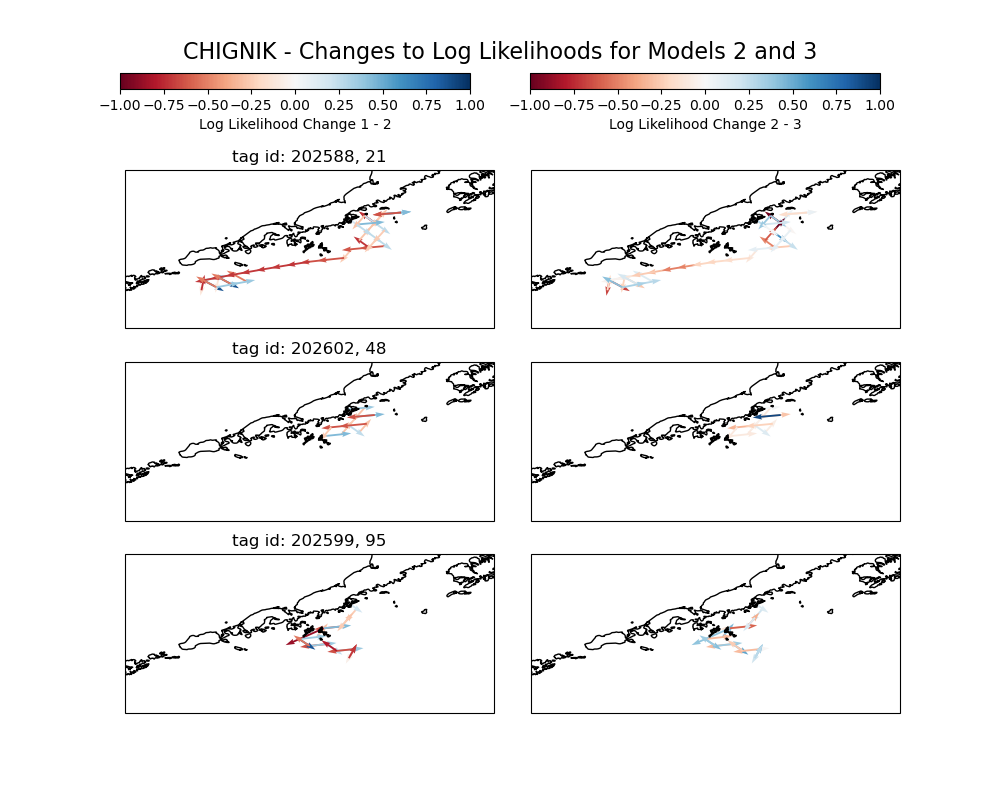
\includegraphics[width=140mm]{figures/chignik_map.png}
  \caption{Log likehood changes per decision - Chignik}
  \label{fig:chignik_map}
\end{figure}

\begin{figure}[h!] 
	\centering
  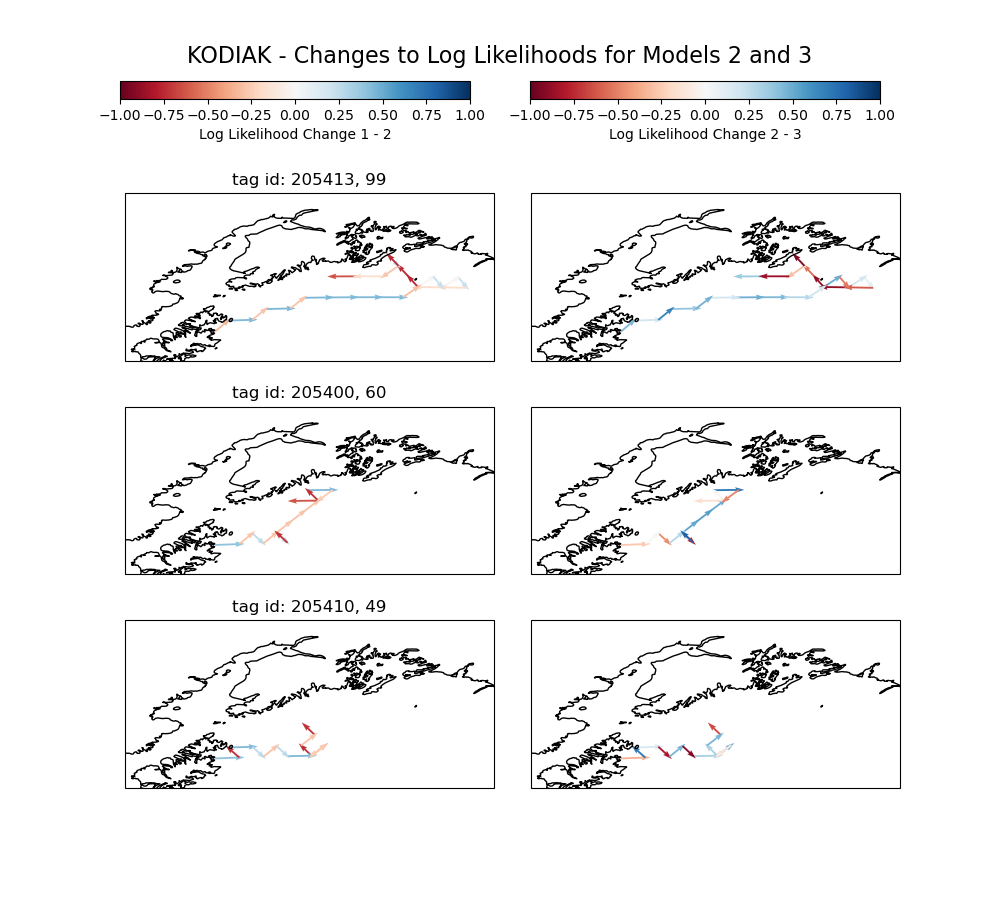
\includegraphics[width=140mm]{figures/kodiak_map.png}
  \caption{Log likehood changes per decision - Kodiak}
  \label{fig:kodiak_map}
\end{figure}

\begin{figure}[h!] 
	\centering
  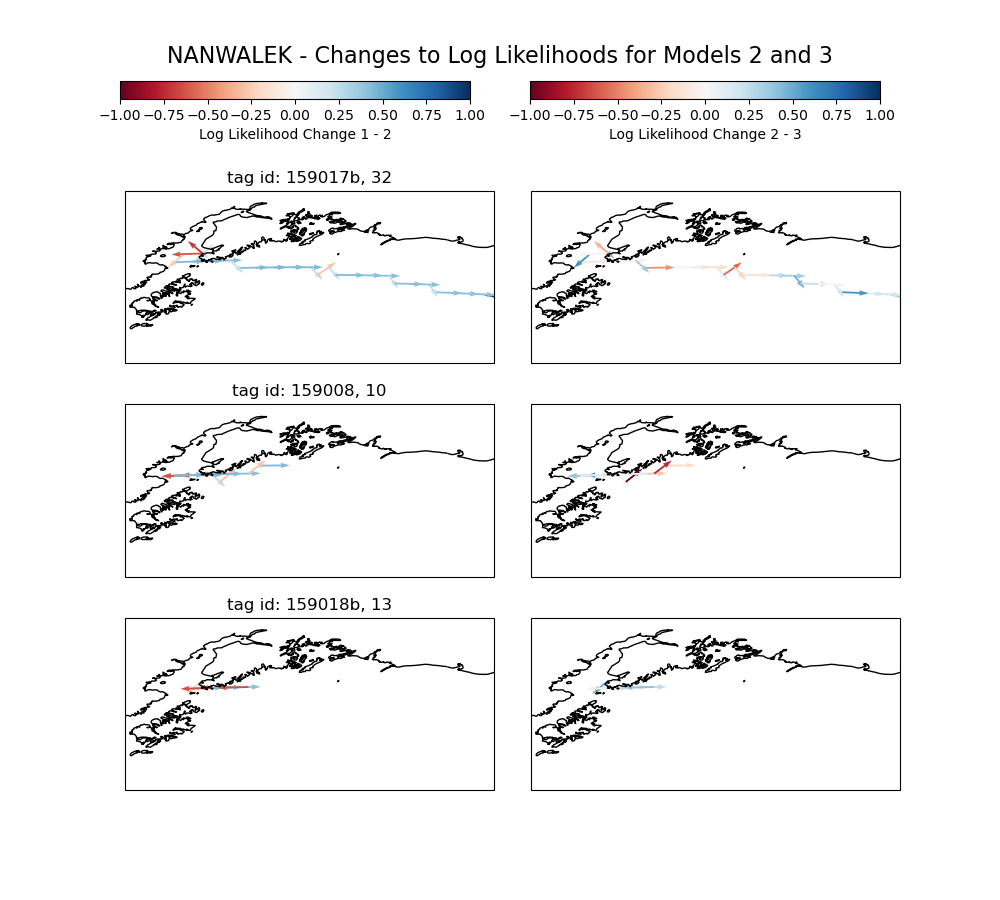
\includegraphics[width=140mm]{figures/nanwalek_map.png}
  \caption{Log likehood changes per decision - Nanwalek}
  \label{fig:nanwalek_map}
\end{figure}

\begin{figure}[h!] 
	\centering
  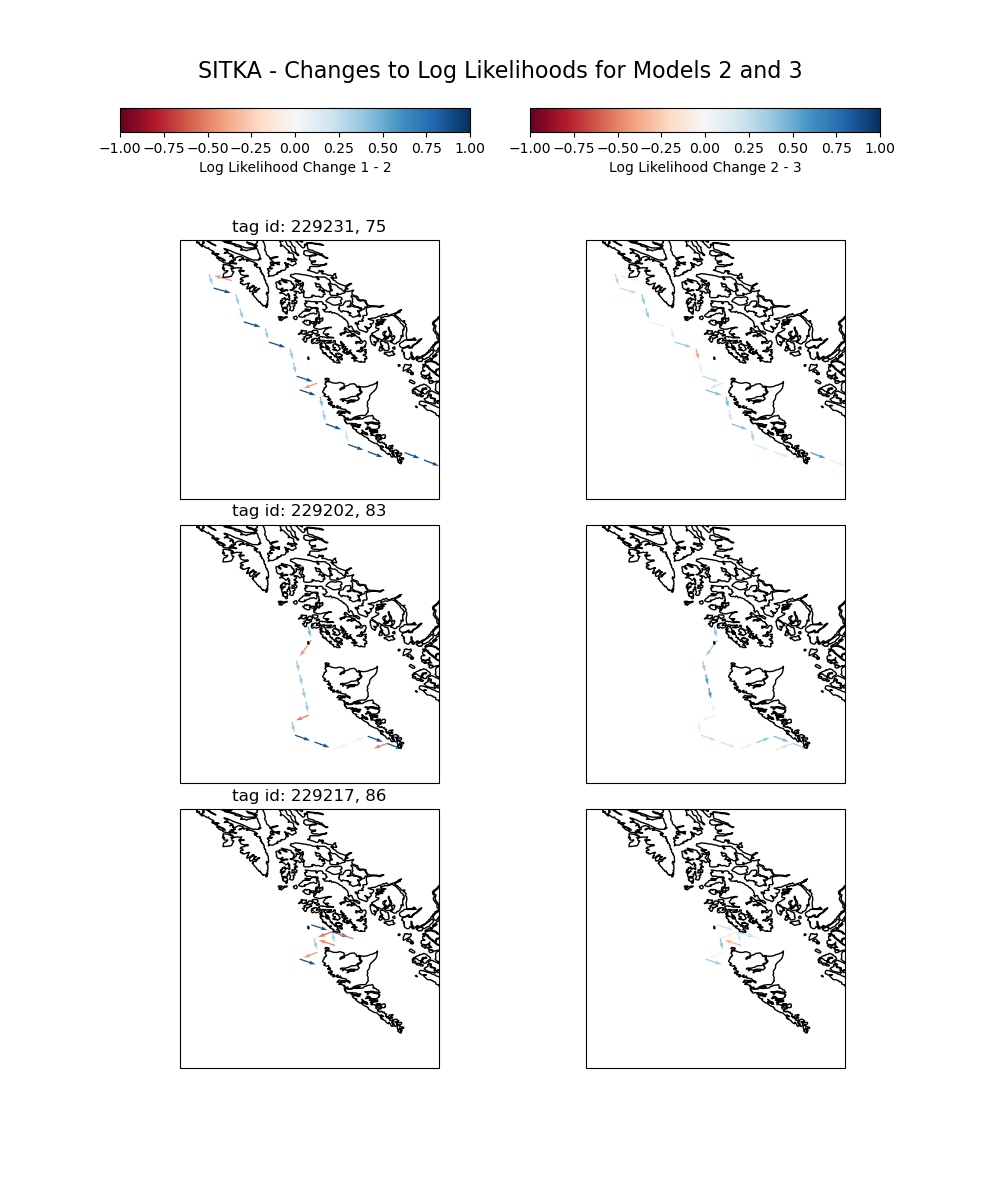
\includegraphics[width=140mm]{figures/sitka_map.png}
  \caption{Log likehood changes per decision - Sitka}
  \label{fig:sitka_map}
\end{figure}

\begin{figure}[h!] 
	\centering
  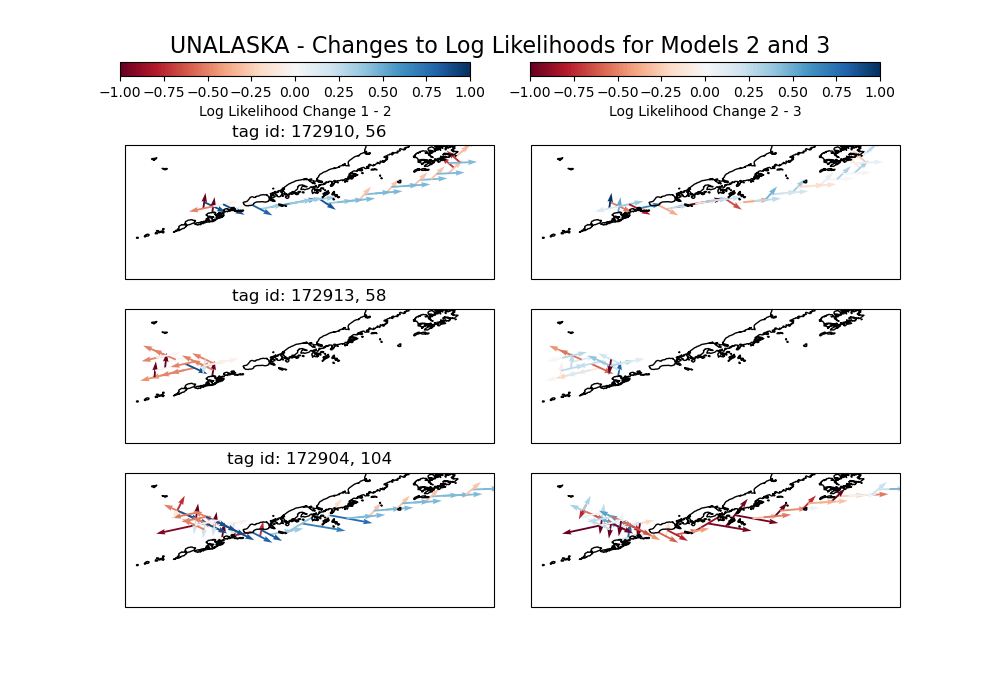
\includegraphics[width=140mm]{figures/unalaska_map.png}
  \caption{Log likehood changes per decision - Unalaska}
  \label{fig:unalaska_map}
\end{figure}

\begin{figure}[h!] 
	\centering
  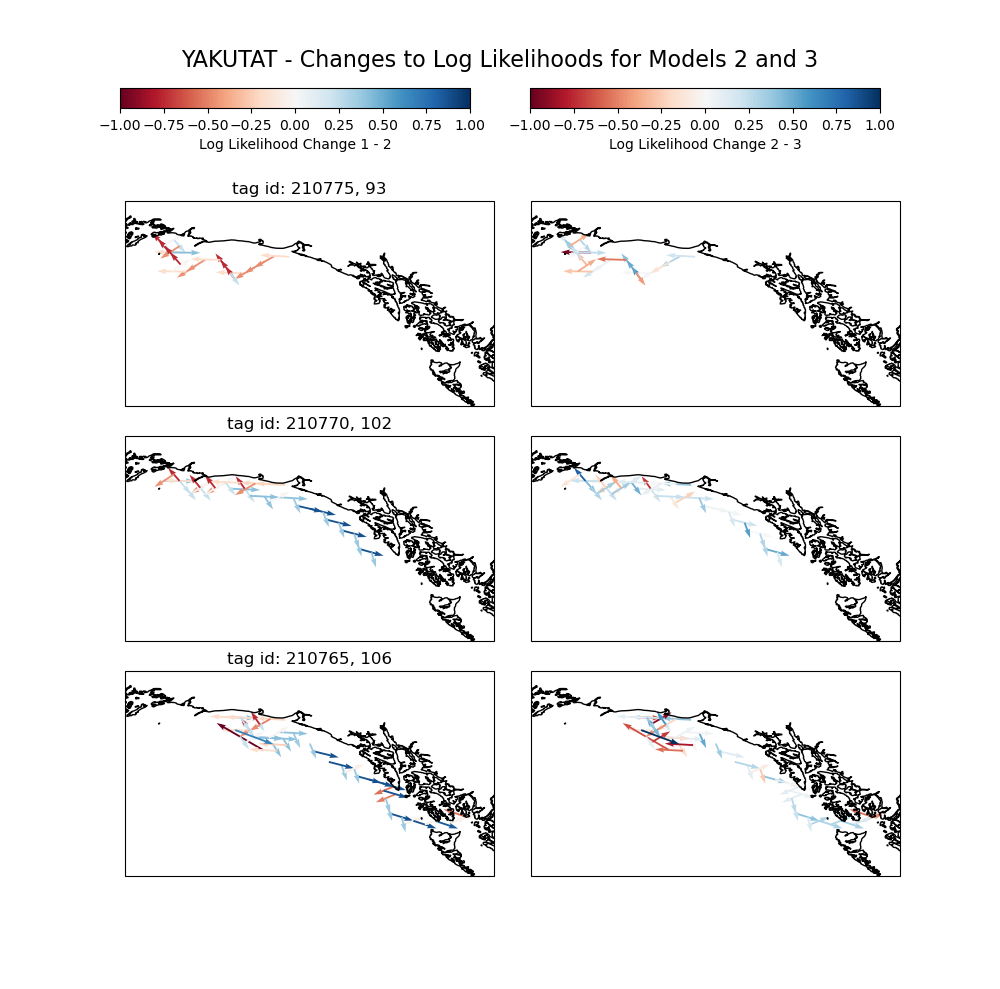
\includegraphics[width=140mm]{figures/yakutat_map.png}
  \caption{Log likehood changes per decision - Yakutat}
  \label{fig:yakutat_map}
\end{figure}

\end{document}